\newcommand{\deriv}[3][]{% \deriv[<order>]{<func>}{<var>}
  \ensuremath{\frac{\partial^{#1} {#2}}{\partial {#3}^{#1}}}}
\newtheorem{theorem}{Theorem}[section]

\chapter{A Dynamical Recipe for Cosmological Disks}\label{ch:background}
\newpage

This chapter provides an overview of the background theory needed to understand subsequent chapters. In Chapter~\ref{ch:introduction}, we discussed simulations of galaxies being critical to having a theoretical understanding of cosmology and galaxy formation. The word ``simulation" was used without fully contextualizing its significance and meaning. We provide that context in \S\ref{sec:motivation}, where we describe what is actually being done when a simulation is run. In \S\ref{sec:galaxy_ics}, we talk about how to apply this theory to study the evolution of equilibrium galaxies.  We talk about  the implications of cosmology in detail in \S\ref{sec:cosmology}, and explain how this specifies an extended view of the discussion in \S\ref{sec:motivation}. This includes how we identify cosmic substructure and the techniques we use for analyzing the time-evolution of disk-derived quantities. 
\section{Physical Motivation of Modelling} \label{sec:motivation}

The goal of this section is to convey to the reader what we mean by a simulation of a galactic system. 

\subsection{Thermodynamics of Self-Gravitating Systems}

The baryonic mass of the Milky Way is largely concentrated in its stars. To first order, the dynamical behavior of the Milky Way is determined by stellar material and dark matter \citep{BM}. While the evolution of gas is governed by the Euler equations with an equation of state, modelling in galactic dynamics requires that we understand how stars and dark matter behave. 

We begin by suggesting a model of a galaxy composed only of a very large number of stars and dark matter, where all stars have the same mass. We call the probability of a star being a specific position, $\textbf{r}$, and velocity $\textbf{v}$, at a time, $t$, the distribution function (DF), $f(\textbf{r},\textbf{v},t)$. The stars and dark matter sit in a combined gravitational potential, $\Phi(\textbf{r})$, in some near-equilibrium state. To fully describe this model, we need to understand how an ensemble of self-gravitating particles gives rise to an equilibrium distribution of stars and dark matter.

Unlike gas, which can exchange thermodynamic energy with itself through a variety of mechanisms, stars and dark matter interact only through gravity. Gravity is a long range force. In fact, the majority of the contribution to the forces on stars in galaxies comes from far outside their immediate neighborhoods (that is to say gravitational energy in non-extensive) \citep{BT}. 

This has a number of interesting implications. Classical equilibrium statistical mechanics tries to understand distributions of particles as ensembles with a given thermodynamic potential. Some commonly used ensembles are the microcanonical ensemble, where $f_0(\textbf{r},\textbf{v})$, the equilibrium state, is determined by holding energy fixed in a closed system, and the canonical ensemble which finds $f_0$ holding the temperature of the system fixed \citep{sethna}. These ensembles break down when non-extensive forces are involved (in the latter case, specifically because self-gravitating systems have no maximum entropy) \citep{self_gravitating_statistical_mechanics,lb_negative_specific_heat, BT}. Another peculiarity of self-gravitating systems is that they have a negative heat capacity \citep{lb_negative_specific_heat}.

The implication is that self-gravitating systems of stars, which have no means to dissipate internal energy, can never be in thermodynamic equilibrium. A system which starts in dynamical equilibrium evolves to a state of higher entropy when perturbed, which is physically characterized as having a dense core and extended envelope of mass \citep{BT}. Since a thermodynamic resolution of galactic dynamics is unattainable, a dynamical theory of galaxy evolution must be developed\footnote{For more information on the thermodynamics of self-gravitating systems, Chapter~4.10 of \citet{BT} and Chapter~7.3 of \citet{BT} provide excellent summaries.}.

\subsection{The Collisionless Boltzmann Equation}

To provide a time-dependent dynamical prescription for our model of stars and dark matter particles, we will make a number of assumptions that hold for the entire thesis. These are:

\begin{itemize}
\item Galaxies are collisionless systems; one does not have to worry about energy exchanged in close encounters because close encounters of individual stars and dark matter particles seldom happen.
\item All stars and dark matter particles are identical.
\item Phase space probability is conserved.
\item Phase space probability is incompressible.
\end{itemize}
We want to turn the assumptions listed above into a solvable equation for $f(\textbf{r},\textbf{v},t)$. This is done by recognizing that  for $\textbf{w} = (\textbf{p}, \textbf{q})$ \citep{BT},
\begin{equation}
\deriv{f}{t} + \deriv{}{\textbf{w}} \cdot \left( f \dot{\textbf{w}}\right) = 0
\end{equation}
is the continuity equation in 6D phase space that expresses conserved phase space probability. Here, $\textbf{p}$ and $\textbf{q}$ are any set of canonical coordinates. In general, this may be rewritten in what is commonly called the Collisionless Boltzmann equation (CBE),
\begin{equation}
\deriv{f}{t} + \dot{\textbf{q}} \cdot \deriv{f}{q} + \dot{\textbf{p}} \cdot \deriv{f}{p} = 0.
\end{equation}
The CBE is more commonly expressed in Cartesian coordinates as,
\begin{equation}
\deriv{f}{t} + \textbf{v} \cdot \deriv{f}{\textbf{x}} - \deriv{\Phi}{\textbf{x}} \cdot \deriv{f}{\textbf{v}} = 0, \label{eq:cbe_cartesian}
\end{equation}
where $\Phi$ is our total gravitational potential from stars and dark matter. The result is a quasilinear partial differential equation (PDE) for $f(\textbf{r},\textbf{v},t)$. The CBE is nothing more than an advection equation in phase space that expresses our view that particles are not self interacting, that they are identical, and that the phase space fluid is conserved and incompressible. In addition to the CBE which describes the evolution of the phase fluid, we have the Poisson equation, an elliptic equation describing the evolution of the potential \citep{BT},
\begin{equation}
\nabla^2 \Phi(\textbf{r},t) = 4 \pi G \rho(\textbf{r},t) \label{eq:poisson}
\end{equation} 
where $G$ is Newton's gravitational constant, $\rho$ is the mass density and,
\begin{equation}
\nu(\textbf{r},t) = \int_{\mathcal{D}} f(\textbf{r}, \textbf{v}, t) \text{d}^3 \textbf{v},
\end{equation}
where $\nu$ is the number density and $\mathcal{D}$ is the phase space. Note that the mass density and number density differ by a factor of the system mass. We are left with a 6D space + 1D time solution domain on which to compute $f(\textbf{r},\textbf{v},t)$ as well as two PDEs and an integral.

\subsection{Monte Carlo Solution of the Collisionless Boltzmann Equation}

In terms of actually solving the CBE, we run into a number of technical challenges in applying traditional finite difference and finite volume schemes for advection equations. These techniques require that some mesh be constructed, and the flows between the cells in the mesh are calculated dependent on the type of equation being solved and the current states of the cells\footnote{Chapter~19 of \citet{numerical_recipes_fortran} discusses numerical methods for PDEs, although you could find detailed discussion of finite difference and finite volume methods in most numerical methods texts.}. The spatial domain is 6D, meaning a uniform mesh resolution scales in memory consumption as $O(N^6)$, where $N$ is the number of cells on an axis. For a sanity check, a modest $N = 2^5$ element grid would take up $2^{30} \times 2^4 \text{ bytes} \sim 17 \text{ GB}$. We obviously need more than 32 cells on an axis to represent the fine DF structure we want to study, and we are already at the limit of a single compute node to apply a finite difference scheme. 

This is where Monte Carlo methods shine. The fundamental principle on which they operate is that I can evaluate the integral of any function, $f(\textbf{x})$, over a domain $\mathcal{D}$, as \citep{numerical_recipes_fortran},
\begin{equation}
\int_\mathcal{D} f(\textbf{x}) d^{n} \textbf{x} = \frac{V(\mathcal{D})}{\vert X_s \vert} \sum_{\textbf{x}_i \in X_s(\mathcal{D})} f(\textbf{x}_i)
\end{equation}
where $X_s$ is a uniform random sample of points on $\mathcal{D}$, $V(\mathcal{D})$ is the volume of the domain, $n$ is the dimensionality of $\textbf{x}$, and $\vert X_s \vert$ is the cardinality, or number of points in the sample. The benefit of Monte Carlo integration is that although our result is not deterministic, the error in the integral is reduced as $1/\sqrt{N}$ \textit{regardless of the integral's dimension}! 

The point of introducing this powerful concept is simply in recognition of the fact that we need to integrate over phase space to solve Eq. \eqref{eq:cbe_cartesian}. As we stated, computing these integrals on a mesh is intractable, so we represent $f(\textbf{r},\textbf{v},t)$ in another way:
\begin{equation}
f(\textbf{r},\textbf{v},t) \approx \sum_i m_i \delta^3(\textbf{r} - \textbf{r}_i) \delta^3(\textbf{v} - \textbf{v}_i)
\end{equation}
where $\delta^3$ is the 3D Dirac delta function, and we take the DF to be normalized to $M = \sum_i m_i$ instead of 1. We call this the N-body realization of the DF. As an extension of this idea, to find $f(\textbf{r},\textbf{v},t)$ at some point in the future, it is sufficient to find the state of our \textit{approximation}\footnote{The author believes that this is one of the most beautiful results ever to be applied in studying the dynamics of galaxies.} at some time in the future. This requires a more detailed exploration of how we step through time with N-body realizations.

\subsection{Time Integration in N-Body Simulations} \label{ssec:time_int}

We have shown how to map solving the CBE, the master equation for our system of stars and dark matter, to the evolution of a finite sample of particles. The system of equations we need to solve now is,
\begin{eqnarray} \label{eq:nbody_system}
\dot{\textbf{r}}_i(t) &=& \textbf{v}_i(t)\\
\dot{\textbf{v}}_i(t) &=& -\left.\deriv{\Phi}{\textbf{r}}\right\vert_{\textbf{r} = \textbf{r}_i}.
\end{eqnarray}
where $\dot{\textbf{r}_i}$ and $\dot{\textbf{v}}_i$ are the first time derivatives of $\textbf{r}_i$ and $\textbf{v}_i$, respectively. Our integro-differential equation system is now approximated as $6\,N$, where $N$ is the number of particles sampled to represent the stars and dark matter, ordinary differential equations (ODEs). These may be solved by any ODE system solver. There are two competing objectives when deciding on the best way to handle time stepping numerically; the first is that we want to maximize the accuracy of our integration scheme and the second is that we want to minimize the number of evaluations of $-\nabla \Phi$, the force. The latter consideration is a severe constraint because naively, the complexity of evaluating each pairwise force is $O(N^2)$.  Although, as we will see, approximations reduce this complexity to $O(N\,\log \, N)$. We note that finding the forces amounts to solving \eqref{eq:poisson}.

Nonetheless, the force calculation will be the most time consuming aspect of the integration, and we want to minimize the number of evaluations we need. This rules out some commonly used schemes in the Runge-Kutta class of integrators, since they would require four or five calculations of the force on millions of particles \citep{numerical_recipes_fortran}. The open question is how to construct a low-order integration scheme that preserves the Hamiltonian\footnote{In a collisionless system, the Hamiltonian should be conserved \citep{BT}.}.

Define the following drift and kick operators for a forward timestep of $\Delta t$ as \citep{quinn_1997},
\begin{eqnarray}
D_t(\Delta t) : \begin{cases} 
	  \textbf{r}_i & \longrightarrow  \textbf{r}_i + \textbf{v}_i \Delta t\\
      \textbf{v}_i & \longrightarrow  \textbf{v}_i 
   \end{cases},
\end{eqnarray}
and,
\begin{eqnarray}
K_t(\Delta t) : \begin{cases} 
	  \textbf{r}_i & \longrightarrow  \textbf{r}_i\\
      \textbf{v}_i & \longrightarrow  \textbf{v}_i  - \nabla \Phi(\textbf{r}_i) \Delta t
   \end{cases}.
\end{eqnarray}
If the Hamiltonian is separable as $\mathcal{H} = T(v) + V(r)$ for $T$, the kinetic energy, and  $V$, the potential energy, and we are in a Cartesian coordinate system, combinations of these operators approximately preserve the Hamiltonian. This is a property of a class of integrators known as symplectic integrators, whose derivation starts with an assumption of Hamiltonian mechanics. We use the second order Leapfrog scheme implemented in \textsc{Gadget-3}, based on the code in \citet{GadgetCodePaper}. It is specified as,
\begin{equation}
U(\Delta T) = K\left(\frac{\Delta t}{2}\right) D\left(\Delta t\right) K\left(\frac{\Delta t}{2}\right).
\end{equation}
This integration scheme is reasonably accurate with only two force evaluations. It is also symplectic, meaning that the Hamiltonian of the system will not drift. Chapter~3 of \citet{BT} has an excellent comparison of numerical integrators, including the Leapfrog scheme given here.

The final remaining complication for the time stepping portion of solving the CBE is determining the timesteps themselves.  Accelerations and velocities in astrophysical systems vary by orders of magnitude, and the timestep needs to be small compared to the timescales defined by the relevant accelerations. Because some particles experience accelerations on a different magnitude than others, we need an adaptive timestep.

The way that this is commonly implemented, including in \citet{GadgetCodePaper}, is to have a base timestep, $\Delta t_{base}$, for all particles that gets bisected at each level of temporal refinement. That is to say, particles at level 4 are updated four more times than particles at level 2. Suppose the highest level of refinement is $k$. The simulation proceeds in $\Delta t_{base} / 2^{k}$ intervals, with particles at $k - 1$ being updated at half of the timesteps, dividing the number of updates by two up to the coarsest level of temporal refinement. Where multiple levels need updates, particles at the lower levels are updated first.

The level of temporal refinement assigned to a given particle is determined primarily by the acceleration it experiences. That is, for \textsc{Gadget-3} \citep{GadgetCodePaper},
\begin{equation}
\Delta t_i = \min\left(\Delta t_{base}, \left(\frac{2 \eta \epsilon}{\vert \nabla \Phi(\textbf{r}_i) \vert} \right)^{1/2}\right).
\end{equation}
Here, $\eta$ is a free accuracy parameter and $\epsilon$ is the gravitational softening. The gravitational softening is used to prevent numerical overflow when particles rarely have close encounters. It arises from having the acceleration induced from a particle at position $\textbf{r}_i$  be,
\begin{equation}
\textbf{a}_i(\textbf{r}) = -\frac{G m_i}{\left(\vert\textbf{r} - \textbf{r}_i\vert^2 + \epsilon^2\right)^{3/2}}(\textbf{r} - \textbf{r}_i) \label{eq:point_mass}
\end{equation}
Higher choices of $\epsilon$ reduce large errors accumulating due to large forces, but also make the force calculation less accurate.

\subsection{Efficient Force Calculation}

The Leapfrog scheme requires us to compute the force two times. Naively, we would compute a sum over Eq. \eqref{eq:point_mass} for each of the $N(N-1)/2$ unique pairs of positions in $O(N^2)$ time to compute the forces on all particles. This is also intractable, or rather is the limiting factor on how large of a simulation we can run. Methods were developed early on in the history of running N-body simulations to cope with this by approximating the potential.

The first method worth noting for this thesis is the particle mesh technique \citep{hockney_pm, white_pm, klypin_pm}. This technique considers the calculation of forces on a 3D mesh by reducing the calculation to a Fast Fourier Transform (FFT) \citep{numerical_recipes_fortran}. One of the crowning achievements of scientific computing in the 20th century was the rediscovery of an algorithm by J. W. Cooley and John Tukey, originally discovered by Gauss, to compute the Discrete Fourier Transform (DFT) in $O(N\,\log\,N)$ complexity\footnote{What Gauss was doing with recursive DFT algorithms is beyond the author, but in the author's humble opinion, it is expected from the greatest mathematician to ever live.}\citep{fft}. Particle mesh's cloud-in-cell (CIC) algorithm was a part of a flurry of algorithms that subsequently exploited the FFT. It has a difficult time accounting for forces from particles separated by small scales on the mesh, though \citep{GadgetCodePaper}.

Compensating for some of the shortcomings of the particle mesh approach, \citet{barnes_hut} introduced a new algorithm for approximating forces in $O(N \,\log\, N)$ complexity. Their algorithm took a divide an conquer approach by subdividing the simulation space into octants recursively until each particle was in its own cell. Forces would be computed pairwise for particles close together, but for distant particles, the mass distribution would be approximated as a multipole. To compute the forces, one simply does a depth-first-search (DFS) of the particle tree, going deeper if,
\begin{equation}
\frac{l}{d} \geq \theta
\end{equation}
where $l$ is the side length of the node whose force is being computed, $d$ is the distance from this node to the current node in the DFS, and $\theta$ is a threshold called the opening angle. In the simplest case, a cell not meeting this condition would be approximated as a point mass with the position at the  center of mass of all particles deeper in its subtree. Higher order multipole expansions are typically used (4 and 8 are common choices).

In addition, the somewhat simplistic opening angle scheme is expounded upon by some codes to include a ``relative opening criterion". The main idea is to use the last acceleration of the particle to determine whether or not a cell needs to be opened. \textsc{Gadget-3} uses the criterion,
\begin{equation}
\frac{G M}{d^2} \left(\frac{l}{d}\right)^2 \geq \alpha \vert\textbf{a}_{i,t-1} \vert
\end{equation}
where $M$ is the mass in the current DFS subtree, $\vert\textbf{a}_{i,t-1} \vert$ is the magnitude of the acceleration of the current particle at the last time step, and $\alpha$ is a relative opening criterion, a free parameter. Conceptually, this means that if the point mass acceleration in the current subtree is greater than a specified fraction of this particle's acceleration, the current DFS level is too coarse and we need to go deeper.

The scheme proposed by \citet{barnes_hut} is widely used in astrophysics because of its efficiency and computability. While both algorithms are $O(N\,\log\, N)$ complexity, tree-based methods tend to perform more slowly in practice \citep{GadgetCodePaper}. \citet{xu_treepm} introduced a scheme to combine both the short-range accuracy of tree methods with the efficiency of FFT-based methods. This TreePM method has been widely successful at handling short range forces with a tree method and long range forces with particle mesh techniques. The trick is forcing consistency between the two methods at intermediate distances. \textsc{Gadget-3} combines a high degree of optimization with the TreePM algorithm to produce a highly efficient algorithm.

Before proceeding to talk about the complications of executing TreePM on distributed systems like the Linux clusters worked with in this thesis, we would be remiss in not mentioning field expansion methods. Typically these take the form of an expansion of the potential in spherical harmonics using a set of radial basis functions. A brief discussion of these methods is presented in Chapter~2.9.4 of \citet{BT}. These methods have great historical significance, and have even seen a recent resurgence in helping understand the structure of dark matter halos \citep{lilley_2018_a, lilley_2018_b}.

To summarize, there are a number of ways to find gravitational forces in a simulation that all amount to solving Poisson's Equation, \eqref{eq:poisson}. The most accurate way is to compute all pairwise forces, but efficient algorithms have been developed to accurately estimate forces from gravity. The force calculation together with a time stepping scheme for N-body realizations forms the main components of an N-body simulation, and solving Eq. \eqref{eq:nbody_system} to estimate $f(\textbf{r},\textbf{v},t)$ is what we mean when we say we ran a simulation.

\subsection{Complications on Distributed Systems}

\begin{figure}
	\centering
	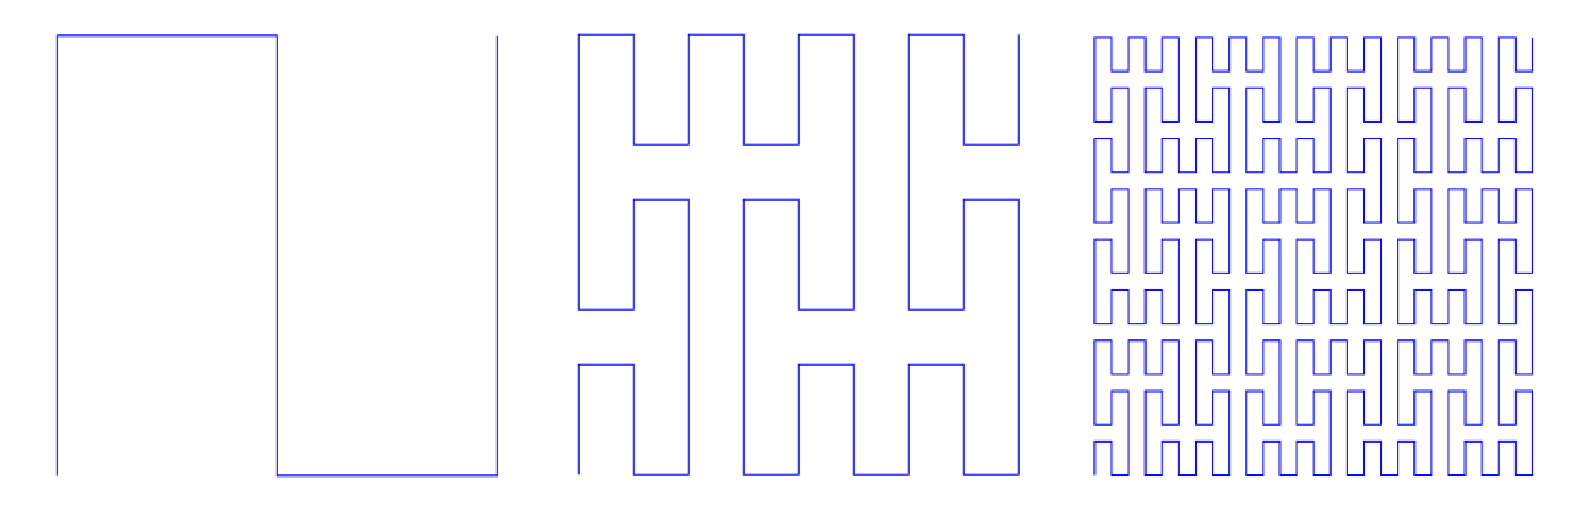
\includegraphics[width=\textwidth]{../figures/Peanocurve.eps}
	\caption{Several examples of the Peano space filling curve in 2D. The level of refinement increases left-to-right. Obtained from \citet{peano}.}\label{fig:peano}
\end{figure}

Modern high performance computing is largely done on compute clusters which are groups of smaller computers (nodes) connected with some high speed connection (Gigabit Ethernet, InfiniBand). The nodes form a distributed system in the sense that they do not share memory addresses. Each node may have multiple processes running (typically up to the number of logical cores on the node's CPU). Processes do not share data\footnote{Processes do not share data in a fully distributed model of parallel computing. Shared memory models like OpenMP \citep{openmp} share data between processes on a single node. MPI 3 even has similar shared memory support \citep{mpi3_shared}. \textsc{Gadget-3} was initially designed to not use these paradigms, and our intention is not to give a complete overview of all of parallel computing, so we relegate clarification to this footnote and references.}, and must communicate through a protocol like the Message Passing Interface (MPI) \citep{mpi_standard}.

Specifically, in an N-body simulation,  will have a subset of all of the particles, and a subset of the total tree structure. A naive DFS of an Octree simply cannot be done since no process will have all of the particles. When a process requires particles from another process, this reduces the efficiency gained from increasing the number of processors, and one might even get an overall slowdown. Another potential problem is that an individual process may get a higher work load than other processes, causing the other processes to wait for it to finish. We talk about how both of these problems are solved here.

To reduce the need to explicitly transfer particles between processes, \textsc{Gadget-3} notes that pairwise forces will only be needed for nearby particles. These represent the bulk of the tree force calculation. Any scheme which puts nearby particles on the same processor will reduce the overall communication time in the force calculation phase. One way to accomplish efficient load balancing is to partition the simulation space using a space filling curve. Fig. \ref{fig:peano} shows the Peano space-filling curve at several levels of refinement in 2D. This is the curve \textsc{Gadget-3} uses. A level of refinement is selected, and estimates of the computational cost in each cube are added up along the space filling curve to equally distribute the computational load. This results in nearby particles being on the same process, and in the processes having roughly equal work loads. \citet{GadgetCodePaper} shows that this is highly effective at reducing communication cost in the simulation, and it goes into more detail about how TreePM is carried out on distributed systems.


\section{Phase Space, Equilibrium, and Initial Conditions} \label{sec:galaxy_ics}
In \S\ref{sec:motivation} we outlined the underlying theory behind representing stars and dark matter in an N-body simulation. The focus of this thesis is studying the behavior of stellar disks in cosmological environments, and the first step towards that understanding is the construction of a pristine, equilibrium N-body model. Ultimately, in the course of running an N-body simulation, these pristine systems will diverge to higher entropy\footnote{The Shannon entropy is a commonly used measure for self-gravitating systems. See \citet{BT} for more details.} states, initially due to random errors in the N-body representation. Nonetheless, these models give us an understanding of how perfectly unperturbed galaxies will evolve due to the fact that real galaxies are also made of a finite number of particles.

\subsection{Jeans Modelling and the Epicyclic Approximation}

The DF represents the 6D phase space information and completely describes an N-body system. In a simple disk-halo system, there is a flattened axisymmetric component (the disk), and a spheroidal component (the dark matter halo) each with their own DF. These are made self-consistent by the separate DFs' incorporation of their combined gravitational potential. 

However, the DF is not the quantity that is observed in external galaxies. Astronomers are not typically working with a 6D phase space description of the structures they observe. Luminosity (density) profiles are one observable , as well as circular velocities (rotation curves) for disks, and also the spread of line of sight (LOS) velocities of disk stars. A modelling approach that takes our understanding of these observables as input is conceptually easier to understand than a DF which may or may not be unique \citep{BT}.

In this spirit, \citet{jeans_1915}\footnote{Notably before the infamous 1920 Curtis-Shapley debate \citep{curtis_shapley} establishing that so-called ``spiral nebulae" were actually external galaxies.} laid out a framework to describe galaxy evolution in terms of the \textit{moments} of the distribution function. Specifically, the idea is to multiply the CBE (Eq. \eqref{eq:cbe_cartesian}) by $\textbf{v}_i$ or $\textbf{v}_i \textbf{v}_j$ and integrate over the velocity part of phase space. These together yield the second-order Jeans equations \citep{BT},
\begin{eqnarray}
\deriv{\nu}{t} + \deriv{\nu \langle v_i \rangle}{x_i} &=& 0 \\
\nu \deriv{\langle v_j \rangle}{t} + \nu \langle v_i \rangle \deriv{\langle v_j \rangle}{x_i} &=& -\nu \deriv{\Phi}{x_j} - \deriv{\nu \sigma^2_{ij}}{x_i}\label{eq:jeans}
\end{eqnarray}
where $i,j \in (1,2,3)$, $\langle\cdot\rangle$ denotes expectation over $f$, $\mathbb{E}_f[\cdot]$, $\nu$ is the number density of particles, and $\sigma^2_{ij} = \langle v_i v_j \rangle - \langle v_i \rangle \langle v_j \rangle$ is the velocity dispersion tensor. In equilibrium for spherical systems, the second equation is often written as \citep{BT},
\begin{equation}
\deriv{\nu \langle v_r^2 \rangle}{r} + \nu \left(\deriv{\Phi}{r} + \frac{2 \langle v_r^2 \rangle - \langle v_\theta^2\rangle - \langle v_\phi^2 \rangle}{r} \right)
\end{equation}
where $\theta$ is the polar angle, $\phi$ is the azimuthal angle, and $r$ is the spherical radius\footnote{Note a slight abuse of notation. We said that $v_i$ has $i \in (1,2,3)$, but here we use symbols to represent specific coordinate systems. The point is that the indices have three unique values.}. Note that there is only one scalar equation. Symmetries in the velocity dispersion tensor for spherical systems require that the cross moments are zero \citep{BT}. For axisymmetric systems, the equilibrium Jeans equations are often written \citep{BT},
\begin{eqnarray}
\deriv{\nu \langle v_R^2 \rangle}{R} + \deriv{\nu \langle v_R v_z \rangle}{z} + \nu \left(\frac{\langle v_R^2 \rangle - \langle v_\phi^2 \rangle}{R} + \deriv{\Phi}{R} \right) &=& 0\\
\frac{1}{R} \deriv{R \nu \langle v_R v_z \rangle}{R} + \deriv{\nu \langle v_z^2 \rangle}{z}+ \nu \deriv{\Phi}{z} &=& 0\\
\frac{1}{R^2} \deriv{R^2 \nu \langle v_R v_\phi \rangle}{R} + \deriv{\nu \langle v_z v_\phi\rangle}{z} &=& 0
\end{eqnarray}
where $z$ is the Cartesian $z$, $R$ is the cylindrical radius, and $\phi$ is the polar angle. These equations look suspiciously like Euler's equations for fluid dynamics with a missing energy equation. \citet{jeans_1915} did not magically solve the statistical mechanical issues mentioned in \S\ref{sec:motivation}; given a number density and potential, we still have an unknown velocity dispersion tensor with six elements, and only 4 independent equations. In the simplified spherical case, we have three unknown elements and two independent equations.

We have also thrown out information about the DF by using moments and stopping at second order. Higher order Jeans equations can be appended to this system by multiplying the CBE by $v_i v_j v_k$ to obtain the third order equations, and so on. These get progressively more complicated, and we would require more additional equations to evaluate the equilibrium Jeans equations \citep{BT}.

Despite these shortcomings, more information can be imposed on the system to make these equations applicable. \citet{hernquist_1993} presented one of the first successful applications of Jeans modelling to creating equilibrium galaxies with bulges, disks, and dark matter halos. In the case of the dark matter halo for a disk-halo system, one only has to specify the function,
\begin{equation}
\beta(r) = 1 - \frac{\langle v_\theta^2\rangle + \langle v_\phi^2 \rangle}{2 \langle v_R^2 \rangle}.
\end{equation}
This parameter measures anisotropy in the velocity ellipsoid defined by $\sigma_{ij}$ at each radius; $\beta = -\infty$ if all orbits are circular, $\beta=0$ if the system is isotropic, and $\beta = 1$ if orbits are purely radial. Together with an assumed density-potential pair, continuity equation, and the spherical second-order Jeans equation, the spherical halo's velocity structure is specified. At the time of writing, \citet{hernquist_1993} did not have much information about the dark matter distribution in galaxies (recall \citep{nfw} proceeded this work in establishing a common density profile for dark matter halos). As such, we will not talk about their uninformed choice of halo, and it really is not important.

In the case of the axisymmetric disk, \citet{hernquist_1993} based their model on the observations at the time which suggested that stellar disks had an exponential radial density profile \citep{freeman_1970}. This motivated a density profile commonly used today,
\begin{equation}
\rho_d(r) = \frac{M_d}{4 \pi R_d^2 z_d} e^{-R/R_d} \text{sech}^2\left(\frac{z}{z_d} \right). 
\end{equation}
Here, $M_d$ is the mass of the disk, $R_d$ is the radial scale length, and $z_d$ is the vertical scale length.
Observations support the idea that the second radial velocity moment also has an exponential profile \citep{van_der_kruit_searle_1981, lewis_freeman_1989},
\begin{equation}
\langle v_R^2 \rangle = \sigma_{R,0} e^{-R/R_\sigma}.
\end{equation}
Here, $R_\sigma$ is the radial dispersion scale length, and $\sigma_{R,0}$ is a free velocity scale (on the order of 100 km/s for the Milky Way). In  principle, any radial scale length can be used for $\langle v_R^2 \rangle$, but it is generally accepted to be a longer scale length than $R_d$. The vertical dispersion and second velocity moment are determined from the assumption of the disc being isothermal,
\begin{equation}
\langle v_z^2 \rangle = \pi G \Sigma z_d
\end{equation}
where $\Sigma_d$ is the surface density as a function of radius. Finally, a relation between $\langle v_\phi^2 \rangle$ and the other second moments is needed to fully solve the second order system. Jeans modelling for discs injects the intuition behind a theoretical development known as the \textit{epicycle approximation}. 

The main idea is that stars in discs are on roughly circular and planar orbits, so a reasonably accurate description of their orbits can be obtained by taking the equations of motion in a truncated series expansion about a circular orbit at the guiding radius, $R_g$. This is better understood in terms of the effective potential in the rotating reference frame in which a star rotating at $R_g$ is stationary. For a star on the $x$-axis, the $\hat{x}$ direction represents the radial direction, the $\hat{y}$ direction is the same as $\hat{\phi}$ in the original frame, and $\hat{z}$ is unchanged. The equations of motion are \citep{BT},
\begin{eqnarray}
\frac{\text{d}^2x}{\text{d} t^2} &=& \deriv{\Phi_{eff}}{R}\\
\frac{\text{d}^2y}{\text{d} t^2} &=& 0\\
\frac{\text{d}^2z}{\text{d} t^2} &=& \deriv{\Phi_{eff}}{z}
\end{eqnarray}
where $\Phi_{eff} = \Phi(R,z) + L_z^2/2 R^2$ is the effective potential in the accelerating (rotating) reference frame, and $L_z$ is the $z$-component of the angular momentum. These equations can be written in a first order expansion as,
\begin{eqnarray}
\frac{\text{d}^2x}{\text{d} t^2} &=& \kappa^2 x\\
\frac{\text{d}^2y}{\text{d} t^2} &=& 0\\
\frac{\text{d}^2z}{\text{d} t^2} &=& \nu^2 z
\end{eqnarray}
where,
\begin{equation}
\kappa^2(R_g) = \left(R \deriv{\Omega^2}{R} + 4 \Omega^2\right)_{R=R_g,z=0},
\end{equation}
with the circular frequency $\Omega$,
\begin{equation}
\Omega^2(R_g) = \frac{1}{R_g} \left(\deriv{\Phi}{R}\right)_{R=R_g,z=0} = \frac{L_z^2}{R_g^4},
\end{equation}
and,
\begin{equation}
\nu^2(R_g) = \left(\deriv{\Phi}{z}\right)_{R=R_g,z=0}.
\end{equation}
That is, a star's orbit is described by three frequencies: its rotational frequency $\Omega$, a radial oscillation frequency, $\kappa$, and a vertical oscillation frequency, $\nu$. This view is accurate so long as the vertical motion does not deviate far from the disc midplane. The actual values of these constants in Galactic astronomy are related to a problem known as the \textit{Oort Problem}, and we believe that for the Sun \citep{BT},
\begin{eqnarray}
\frac{\kappa}{\Omega} &\approx& 1.35 \\
\frac{\nu}{\kappa} &\approx& 2
\end{eqnarray} 
The fact that the orbit is described by three distinct frequencies that are unequal for the Sun means that the Sun's orbit does not close. If the Milky Way potential never changed, the path of the Sun would fill an annulus centered around $R_g$ \citep{BT}. That is to say, the orbit looks like it forms a rosette pattern.

By assuming the epicycle approximation, we are able to form a complete solution to the Jeans equations for the disc. This is done by looking at a dynamical property of disc star orbits called \textit{asymmetric drift}, which is the velocity defined by \citep{BT},
\begin{equation}
v_a = v_c -  \langle v_\phi \rangle
\end{equation}
where $v_c = R \Omega$. We have yet to discuss how we find $\langle v_\phi^2 \rangle$, whose non-zero nature explains why we have asymmetric drift in the first place. By evaluating the asymmetric drift with the assumptions of the epicycle approximation, we get \citep{hernquist_1993},
\begin{equation}
\sigma_\phi^2 = \langle v_\phi^2 \rangle = \langle v_R^2 \rangle \frac{\kappa^2}{4 \Omega^2},
\end{equation}
where the fraction in the product contains quantities solely determined from the potential, and the coefficient is determined from the assumed radial dispersion profile. This fully solves a disc-halo system. In practice, the system is realized by sampling the spatial density profile (by rejection sampling, for instance) and assigning velocities assuming Gaussians with means $\langle v_i \rangle$ and variances $\langle v_i^2 \rangle$. 

\subsection{DF-based Models and the Jeans Theorem}

Although Jeans modelling is used to set up initial conditions for galaxies because it does not require a DF to be known ahead of time, the best initial conditions are generated from DFs \footnote{That is not to say that no one uses Jeans modelling to set up ICs. Approaches like the one presented in \citet{hernquist_1993} were enormously successful and still used today.}. In general, the equilibrium DF is a function of six variables. However, there are some quantities, called \textit{integrals of motion}, which do not change along a star's orbit in a potential. For an axisymmetric potential, these are the total energy, $\mathcal{E}$, $L_z$ and a third quantity, $I_3$.  
For spherical systems, up to five integrals of motion are admitted by the system, but the simplest \textit{ergodic} models simply have $f_{h}(\mathcal{E})$ for the DF. 


If we assume the epicycle approximation, then $I_3 \approx E_z = \Phi(R,0) - \Phi(R,z) + \frac{1}{2} v^2$, where $v$ is the velocity of an orbit \citep{kd95galactics}. The vertical energy, $E_z$, is conserved so long as the disc is razor thin. Jeans showed that a DF that is a function of the integrals of motion describes an equilibrium distribution. More specifically, quoting from \citet{BT},
\begin{theorem}[The Jeans Theorem]
Any steady-state solution of the collisionless Boltzmann equation depends on the phase-space coordinates only through integrals of motion in a given potential, and any function of the integrals yields a steady-state solution of the collisionless Boltzmann equation.
\end{theorem}
Proof of this theorem can be obtained in \citet{jeans_1915} and in Chapter~4.2 of \citet{BT}, although it essentially amounts to observing that the time derivative of a function of time-independent quantities is zero by the chain rule. Now that we know that any DF of the integrals of motion gives a steady state solution, and that using the epicyclic approximation gives us three known integrals of motion, we can ask ourselves what kinds of DFs describe the NFW haloes and exponential disks that are easily obtained from Jeans modelling.

We talk about the case of an ergodic halo and DF yielding an exponential disc at length here. For the remainder of the thesis, we primarily generate our initial conditions in this way. For any ergodic DF, a chosen density profile may be inverted by the Eddington inversion formula \citep{BT},
\begin{equation}
f(\mathcal{E}) = \int_0^{\mathcal{E}} \frac{\text{d} \Psi}{\sqrt{\mathcal{E} - \Psi}} \frac{\text{d} \nu}{\text{d} \Psi} \label{eq:eddington}
\end{equation}
where $\Psi = - \Phi$. Note that the combined potential need not be spherical, only the overall density of the spheroidal halo. We choose a truncated NFW profile \citep{nfw},
\begin{equation}
\nu_h(r) \sim \rho_{h}(r) = \frac{\rho_0 R_s^3}{r (R_s + r)^2}
\end{equation}
where $\rho_0$ is a scale density and $R_s$ is the halo scale length as our target halo density. By obtaining the 1D DF from Eq. \eqref{eq:eddington}, we can sample halo orbits given the combined disc-halo potential.

For the disc DF, we use a DF that yields exponential discs presented in \citet{kd95galactics}. Noting that if $E_z$ is an integral of motion that $E_p = \mathcal{E} - E_z$ is also an integral of motion, we use,
\begin{equation}
f_d(E_p,L_z,E_z) = \frac{\Omega(R_c)}{(2 \pi^3)^{1/2} \kappa(R_c)} \frac{\tilde{\rho_d}}{\tilde{\sigma_R}^2(R_c) \tilde{\sigma_z}(R_c)} \exp\left[-\frac{E_p - E_c(R_c)}{\tilde{\sigma_R}^2(R_c)}  - \frac{E_z}{\tilde{\sigma_z}^2(R_c)}\right].
\end{equation}
Note that the quantities $\Omega$ and $\kappa$ have their usual definitions, the tilde functions are free choices to tune the disc properties (although they are qualitatively understood as velocity dispersions), and $E_c$ is the energy of a circular orbit. Note that the $R_c$-dependent quantities do not violate the sole dependence on integrals of motion, since $R_c$ is uniquely obtained in a one-to-one fashion from $L_z$.

For the tilde functions, we choose them to yield the closest thing to an exponential-sech$^2$ density profile with and exponential radial velocity dispersion as possible. Assuming an exponential radial dispersion profile, a disc density is obtained by iteratively adjusting $\tilde{\sigma_z}$ and $\tilde{\rho}$ such that \citep{kd95galactics},
\begin{equation}
\rho_d(R,z) = \frac{M_d}{8 \pi R_d^2 z_d} e^{-R/R_d} \text{erfc }\left(\frac{R - R_{out}}{\sqrt{2} \delta R_{out}}\right) \exp \left[ -0.8676 \frac{\Psi_z(R,z)}{\Psi_z(R,z_d)}\right]
\end{equation}
Here, $M_d$ is a parameter that is approximately equal to the mass of the disk, $R_{out}$ is a truncation radius, $\delta R_{out}$ is a parameter determining the sharpness of the truncation, and $\Psi_z$ is the negative vertical potential, $\Phi(R,0) - \Phi(R,z)$. The motivation behind the last term in the product is to yield a dropoff of vertical density close to $\text{sech}^2(z/z_d)$.

Similar to the  Jeans models, we actualize these systems by sampling their combined spatial densities. At every sampled point, we draw a velocity from the DF that is constructed in the combined potential. This does not require us to, for example, use a Gaussian distribution for the velocity dispersions as in Jeans models. This kind of model is as accurate as the assumption that $E_z$ is an integral of motion is (as accurate as the epicycle approximation is). A more detailed discussion about how self-consistent systems are realized from DFs can be found in \citet{kd95galactics}, and this work forms the basis for the \textsc{GalactICS} code used in this thesis.

\subsection{Action-Angle Variables and the Strong Jeans Theorem}

Of course, $E_z$ is only approximately an integral of motion for axisymmetric, nearly planar systems. Although not a substantial element of this thesis, it is worth mentioning a different approach to approximating integrals of motion. Instead of explicitly assuming we are working with an axisymmetric, static system and deducing the conserved quantities, let's ask more generally, \textit{for any system}, what are the conserved quantities? Integrals of motion have the property that orbits may be viewed as single points in a space with dimension of the number of integrals. The only thing unique about them is where they are in the phase of the orbit.

With this in mind, we introduce the actions \citep{BT},
\begin{equation}
\textbf{J} = \oint \textbf{p} \cdot \text{d}^n \textbf{q}
\end{equation}
where $\textbf{J}$ are the actions, and $\textbf{p}$ and $\textbf{q}$ are canonical coordinates. The closed path over which this integral is evaluated yields a unique set of actions. If the system is axisymmetric and the path we have chosen is a circle of radius $R$, it is straightforward to see that the radial component of the action is just $L_z = R v_c$, which depends on the potential. 

Turning the definition of the actions into a transformation from a physically motivated conjugate coordinate system is difficult in general. Closed form solutions for axisymmetric systems exist if the potential if of the St\"ackel form\footnote{For more detail, see Chapter~3.5.3 of \citet{BT}.}, but in general, these transformations do not exist. A commonly used technique is to locally approximate the potential as being of the St\"ackel form \citet{binney_2012}. In practice, one is reduced to approximating the potential instead of the third integral of motion as in the case of \textsc{GalactICS}. For nearly planar disc systems, the differences are insignificant, but become more relevant as one wants to initialize a thicker disc \citep{vasiliev_2018,bauer2018b}.


\section{Cosmology and Implications for Galaxy Studies} \label{sec:cosmology}
Our discussion up to this point has focused on simulating isolated systems. Complications arise when we move to a fully cosmological environment. The purpose of this section is to briefly review relevant cosmology, and to explain what numerical methods must be modified and used to simulate cosmological systems. We conclude this section with a brief commentary on identifying substructure in simulations.

\subsection{Simulations of FRW Cosmology: Large Scale Properties}

In words, the $\Lambda$CDM paradigm described in Chapter~\ref{ch:introduction} prescribes a Universe comprised of four fundamental substances: baryons, radiation, dark matter, and dark energy. On large scales, the Universe is also believed to be isotropic and homogeneous, meaning the patch we occupy is the exact same as any other patch. General Relativity provides a mechanism for us to meaningfully compute distances between patches is this scenario. The so-called Friedmann-Robertson-Walker metric tells us that the \textit{proper distance} between two points at different positions in space and at different times is \citep{kolb_turner, dodelson},
\begin{equation}
\text{d}\,s^2 = c^2 \text{d}\,t^2 + a^2(t) \left(\frac{\text{d}\,r^2}{1 - k r^2} + r^2\text{d}\,\Omega^2 \right).
\end{equation}
Here, $c$ is the speed of light, $t$ is the time coordinate, $a$ is the scale factor of the Universe which is equal to 1 at present day and 0 at the Big Bang, $k$ describes the spatial curvature, and $r$ and $\Omega$ have their standard spherical coordinate definitions. The case used for the whole thesis is where $k=0$, a flat Universe. Assuming this metric, and that all substances in the Universe behave like perfect fluids, it can be shown with General Relativity that the large scale evolution of the Universe is described by the following, the Friedmann Equations \citep{kolb_turner,dodelson},
\begin{eqnarray}
\left( \frac{\dot{a}}{a} \right)^2 &=& \frac{8 \pi G}{3} \rho\\
\frac{\ddot{a}}{a} &=& -\frac{4 \pi G}{3}\left(\rho + \frac{3 p}{c^2}\right).
\end{eqnarray}
Here $\rho$ is the density of the Universe, $p$ is the pressure of the Universe, and we introduce the definition $H(t) = \dot{a} / a$, the Hubble parameter. With the definition of the Hubble parameter, the first of the Friedmann equations is commonly expressed,
\begin{equation}
\left(\frac{H(t)}{H_0}\right)^2 = a^{-4} \Omega_{R,0} + a^{-3} \Omega_{M,0} + \Omega_{\Lambda,0}
\end{equation}
where $\Omega_{R,0}$, $\Omega_{M,0}$, and $\Omega_{\Lambda,0}$ are the relative contributions of radiation, dark and baryonic matter, and dark energy at present day, respectively. Also, $H_0$ is the present-day Hubble parameter. Every flat $\Lambda$CDM universe has these as free parameters, and we can choose them to be anything we like. The different powers of $a$ reflect how radiation, matter, and dark energy contribute differently to the energy as the Universe expands, and can be deduced under relatively few assumptions \citep{kolb_turner,dodelson}.

When simulating a $\Lambda$CDM universe, we can choose to work in a frame where relative distances between fixed points remain fixed. This is the proper coordinate system. The distance between two objects in a proper coordinate system, $d$, for a flat Universe is simply,
\begin{equation}
d(t) = a(t) r \label{eq:comoving_dist}
\end{equation}
where $r$ is the proper distance. An interesting notable consequence of this is,
\begin{eqnarray}
\dot{d} &=& \dot{a} r + a \dot{r} \\
\frac{\dot{d}}{a} &=&  \frac{\dot{a}}{a} r + \dot{r} \\
&=& H(t) r + \dot{r}.
\end{eqnarray}
If two objects are at rest with respect to the proper coordinate system at present day ($\dot{r} = 0$), we measure a non-zero proper velocity,
\begin{equation}
\dot{d} = H_0 r.
\end{equation}
This effect was first described by \citet{hubble_1929}, and explains why distant galaxies appear to be moving away from us. More generally, we call this term in the proper velocity the \textit{Hubble flow}.


% Comoving coordinates and redshift


Following up on this concept, we introduce the notion of \textit{redshift}. The term derives from the fact that as objects become more distant, we expect the hubble flow to cause the emitters to move away from the observer. Photons emitted by a stationary object with a wavelength, $\lambda$, are observed with wavelength $a(t_{emit}) \lambda$, and we define the redshift, $z$,
\begin{equation}
1 + z = \frac{1}{a}
\end{equation}
in analogy to this phenomenon. This is a descending unit of time that is often used interchangeably with the scale factor, $a$.
\subsection{Simulations of FRW Cosmology: Cosmological Initial Conditions}

Of course, the Universe is not actually homogeneous on small scales. As we suggested in Chapter~\ref{ch:introduction}, small scale fluctuations are present in the early Universe which collapse to form galaxies. Initially, these fluctuations evolve independently of each other in the so-called \textit{linear regime}. Initial conditions for $\Lambda$CDM simulations rely on this fact to generate the initial perturbations for the simulation.

The prevailing view in cosmology is that the Big Bang was followed by the development of a primordial perturbation field. As the Universe expanded, interactions with baryons and radiation modified the initial distribution of perturbation scales. Mathematically, we take the the perturbation field $\delta(\textbf{r}, t)$, which describes the deviation from the Universe's mean density at some position and time, and find its Fourier transform. The result is a statistical distribution, called the \textit{power spectrum}, that describes the scale of perturbations \citep{music},
\begin{equation}
P(k) = \alpha k^{n_s} \mathcal{T}^2(k)
\end{equation}
where $\alpha$ is a normalization constant, $n_s$ is a spectral index describing the original inflationary produced perturbations, and $\mathcal{T}$ is a scale-dependent \textit{transfer function} that describes deviations from a power law at different scales. For reference, low $k$ corresponds to larger perturbations in the same way that low frequency corresponds to larger time gaps. The smallest structures occur at high $k$.  

While a detailed discussion of how the transfer function is computed can be found in \citet{music}, we will simply say that it is a reflection of the idea that perturbations only grow when matter becomes dominant. It reflects how we believe that perturbations of different scales grew at different rates in the early Universe. However, once it is known at some desired time (redshift), we can sample a Gaussian density field with the right statistical characteristics. This spatial sample with corresponding velocities obtained via something called 2nd Order Lagrangian Perturbation Theory\footnote{See \citet{music} for a detailed description of this technique.} form the initial conditions for our $\Lambda$CDM simulation.

% Maybe say something about zoom-ins?
\subsection{Extension of Numerical Methods: Time Integration}

Two big problems are present for applying N-body techniques as described. The first, and maybe most obvious of these, is in how we step through time. The time integration scheme worked out in \S\ref{ssec:time_int} makes a critical assumption: the Hamiltonian and its separable components are time independent! Eq. \eqref{eq:comoving_dist} forces us to re-express the leapfrog scheme. For primed quantities as proper (comoving), we have  our new system\citep{quinn_1997},
\begin{eqnarray}
\dot{\textbf{v}^\prime} + 2 H(t) \textbf{v}^\prime &=& -\frac{\nabla^\prime \phi^\prime}{a^3}\\
\dot{\textbf{r}^\prime} &=& \textbf{v}^\prime\\
\nabla^{\prime 2} \phi^\prime &=& 4 \pi G \left(\rho^\prime - \rho_b^\prime \right)
\end{eqnarray}
where $\textbf{r}^\prime$ is the comoving position, $\textbf{v}^\prime$ is the comoving velocity, $\phi^\prime$ is the comoving potential, $\rho^\prime$ is the comoving mass density, and $\rho_b^\prime$ is the mean comoving background mass density. The new drift/kick operators are then defined implicitly \citep{quinn_1997},
\begin{eqnarray}
D_t(\Delta t) : \begin{cases} 
	  \textbf{r}^\prime_i & \longrightarrow  \textbf{r}^\prime_i + \textbf{v}^\prime_i \Delta t\\
      \textbf{v}^\prime_i & \longrightarrow  \textbf{v}^\prime_i 
   \end{cases},
\end{eqnarray}
and,
\begin{eqnarray}
K_t(\Delta t) : \begin{cases} 
	  \textbf{r}^\prime_i & \longrightarrow  \textbf{r}^\prime_i\\
      \textbf{v}^\prime_i & \longrightarrow  \textbf{v}^\prime_i \frac{1 - H(t) \Delta t}{1 + H(t) \Delta t} + \frac{\nabla^\prime \phi^\prime(\textbf{r}^\prime_i) \Delta t}{a^3(t) \left(1 + H(t) \Delta t \right)}
   \end{cases}.
\end{eqnarray}
The problem is that there does not appear to be a way to work forward from a separable Hamiltonian to these operators. Thus, any integration scheme constructed from these operators will not be free of energy drift. To get around this, we ask if there is some canonical transformation that can give us a symplectic integrator. Via a derivation in \citet{quinn_1997}, we find that for a choice of $\textbf{r}^\prime$ as our coordinate system, the canonical momentum is $\textbf{p}^\prime = a^2 \textbf{v}^\prime$. The Hamiltonian is,
\begin{equation}
H = \frac{\textbf{p}^\prime}{2 a^2} + \frac{\phi^\prime}{a},
\end{equation}
for $\phi^\prime = a \phi + \frac{1}{2} \ddot{a} a \textbf{r}^{\prime 2}$. This is a separable Hamiltonian with drift and kick operators,
\begin{eqnarray}
D_t(\Delta t) : \begin{cases} 
	  \textbf{r}^\prime_i & \longrightarrow  \textbf{r}^\prime_i + \textbf{p}^\prime_i \int_{t}^{t + \Delta t} \frac{\text{d}\,t}{a^2(t)}\\
      \textbf{p}^\prime_i & \longrightarrow  \textbf{v}^\prime_i 
   \end{cases},
\end{eqnarray}
and,
\begin{eqnarray}
K_t(\Delta t) : \begin{cases} 
	  \textbf{r}^\prime_i & \longrightarrow  \textbf{r}^\prime_i\\
      \textbf{p}^\prime_i & \longrightarrow  \textbf{p}^\prime_i - \nabla^\prime\phi^\prime \int_{t}^{t + \Delta t} \frac{\text{d}\,t}{a(t)}
      \end{cases}
\end{eqnarray}
Since these operators derive directly from a separable Hamiltonian, this integrator is symplectic. Even though the energy of our cosmological system is not conserved, there will be no drift about the continuum system's actual energy. This is the integration scheme used in \textsc{Gadget-3} for cosmological simulations.

\subsection{Extension of Numerical Methods: Gravity Calculation}

Beyond the coordinate systems and time stepping scheme used in cosmological simulations, there is also the issue that the actual Universe, the system we are trying to simulate, extends over vast distances. Typically, only a box, a few tens to hundreds of Mpc per side is simulated. Gravity is a long range force, and there will be a contribution at any point in the simulation box from distant, massive objects. The way that this handled in modern cosmological simulations is to impose periodic boundary conditions when we solve Poisson's equation. This is essentially like viewing our simulation box cloned infinitely many times along each axis, shifted by its length along each axis.

For forces computed using an FFT-based technique like particle mesh, periodic boundary conditions are assumed. The DFT by its nature implies the density signal in the box repeats forever. For non-grid based techniques, this is not so trivial. Normally, \textsc{Gadget-3} will use a DFT to compute long range forces. However, it does implement a way to use its tree code for long range calculations \citep{GadgetCodePaper}. While for this thesis, the particle mesh grid functionality is used for long range forces, a description of how \textsc{Gadget-3} implements its tree code with periodic boundary conditions can be found in \citet{hernquist_1991}.

\subsection{Identifying Substructure in Simulations}


The picture of a simulated $\Lambda$CDM universe has been conceptually and quantitatively described up to this point. The key concept tying simulations of $\Lambda$CDM to isolated galaxy simulations is the presence of substructure. Here, we describe how we identify substructure in these complicated simulations. 

First and foremost, the question of finding substructure in data is not unique to astrophysics. More generally, we are solving an unsupervised machine learning problem called \textit{clustering}. Solutions to clustering problems take unlabeled data, such as particle masses, positions, and velocities, and identify significant groups within the data \citep{statistical_learning_r}. 

Although there are many techniques that one can use to find clusters in data, we focus on \textit{hierarchical clustering} methods, which as the name suggests, are meant to build hierarchies of clusters. Since $\Lambda$CDM simulations produce subhalos within halos, we expect a such a structure in these clusters.

There are two general approaches to hierarchical clustering \citep{statistical_learning_r}. Agglomerative methods initially place each particle in their own cluster, and will merge two clusters if they meet some kind of \textit{linkage criterium}. For example, given clusters $C_1$ and $C_2$, the complete-linkage approach will merge the two clusters if $\max\left\{ d(c_1, c_2) : c_1 \in C_1 \wedge c_2 \in C_2\right\} < l$, for some distance metric\footnote{Common distance metrics are the Euclidean metric or the Mahalanobis distance \citep{statistical_learning_r}.}, $d$,  and a linking length, $l$ that is a free parameter. Other common metrics include the single-linkage criterion, $\min\left\{ d(c_1, c_2) : c_1 \in C_1 \wedge c_2 \in C_2\right\} < l$, and the average linkage criteria $\langle d(c_1,c_2) \rangle \left (c_1 \in C_1 \wedge c_2 \in C_2\right) < l$.

\begin{figure}[h]
	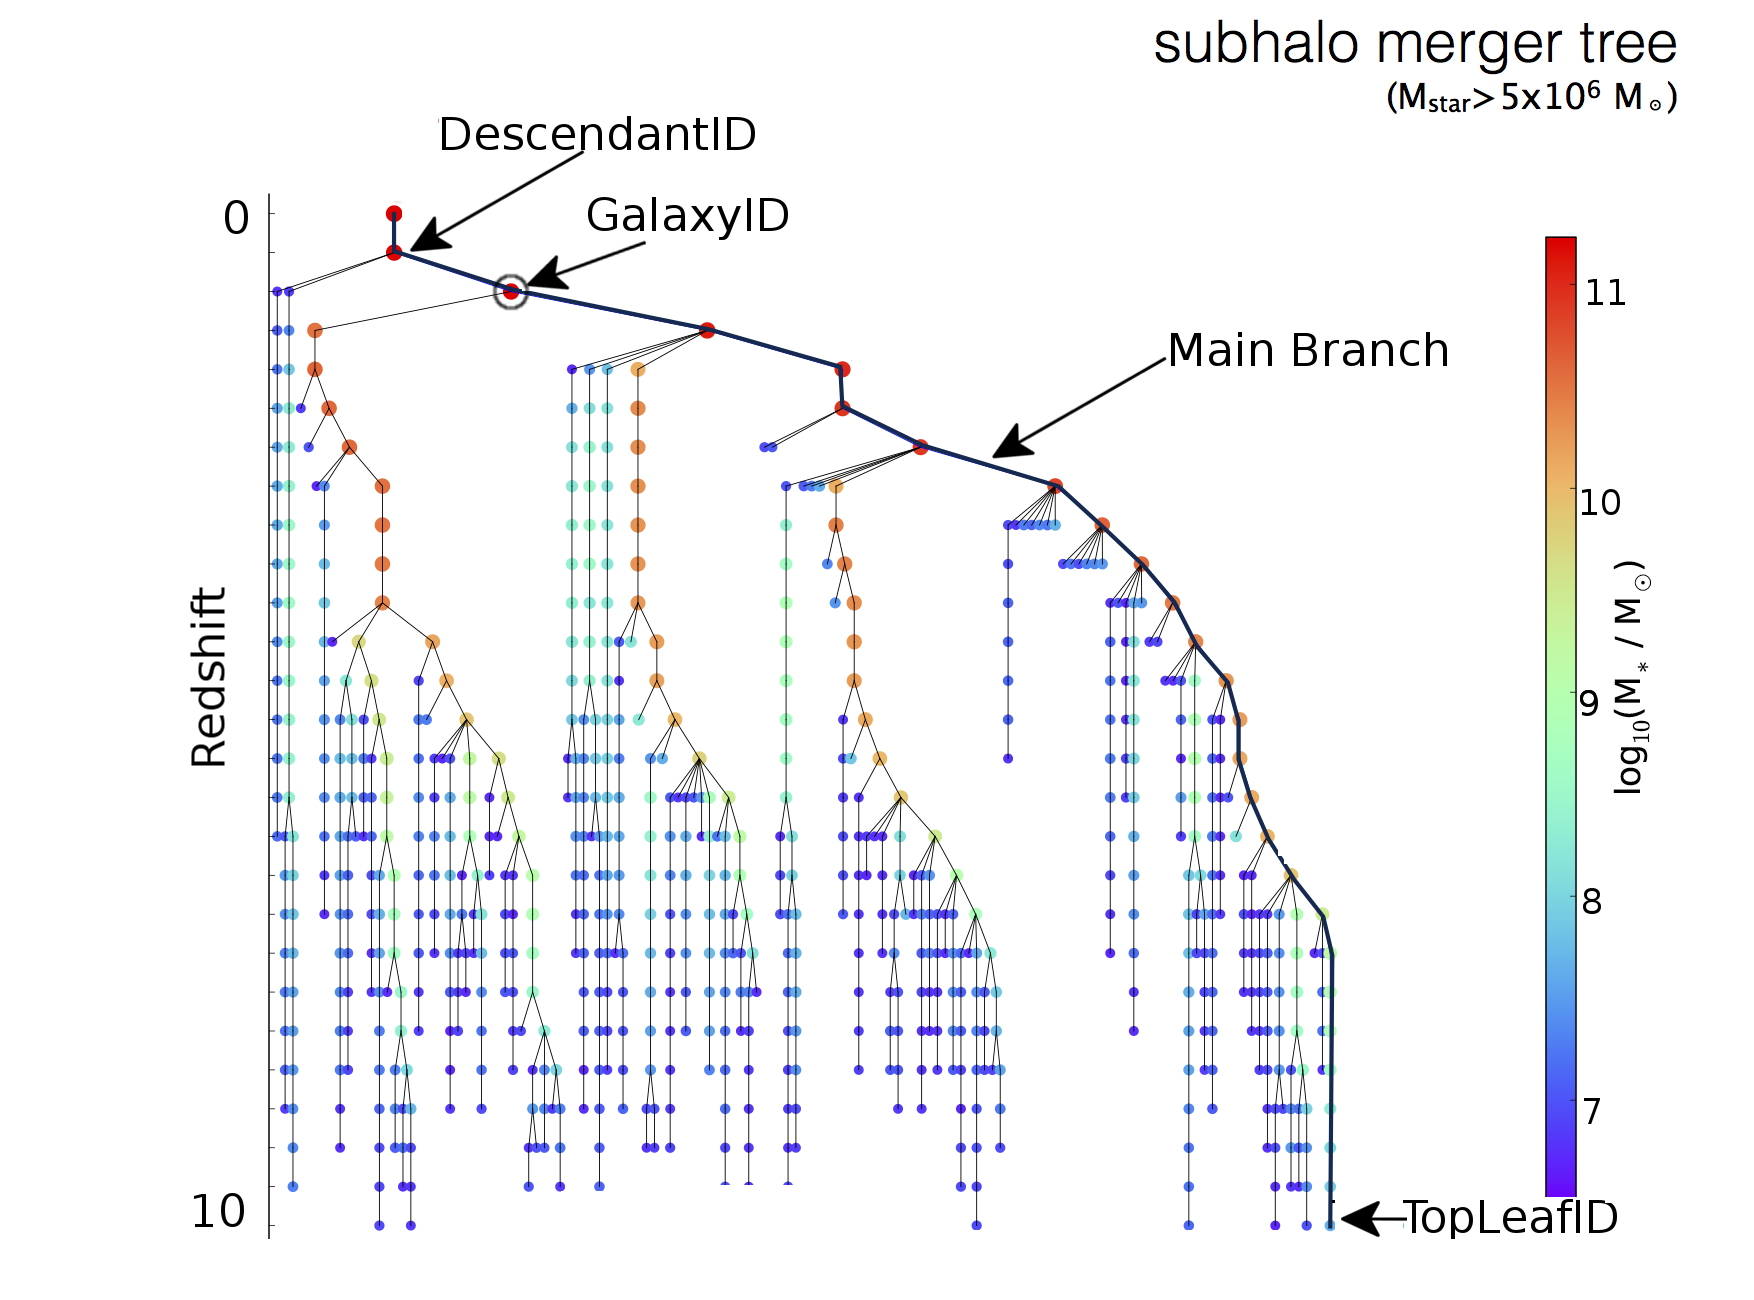
\includegraphics[width=\textwidth]{../figures/eagle_tree}
	\caption{A merger tree obtained from \citet{merger_tree}. It represents the merging history of a halo in a simulation presented in \citet{Eagle}.} \label{fig:merger_tree}
\end{figure}

The other approach to hierarchical clustering is divisive clustering, which starts with all of the particles in the same cluster \citep{statistical_learning_r}. Divisive clustering splits the top cluster into objects of maximum dissimilarity until each object is its own cluster. Here, dissimilarity is defined by some metric chosen ahead of time. 

Regardless of which approach to hierarchical clustering one uses, the end result is a tree-like structure called a \textit{dendrogram}, with large clusters at the top and individual particles at the bottom. In simulations of cosmology, we construct these at every timestep to determine which halos merged with other halos. There is a long literature on this subject described in \citet{rockstar}, although we use their implementation, the \textsc{rockstar} code, in this thesis.

The main idea behind the algorithm implemented in \textsc{rockstar} is to first apply a divisive scheme to the 3D data to create more manageable subclusters that get piped to an agglomerative 6D scheme. A big issue in the literature has been finding distance metrics which work with 6D phase space information in an acceptable manner \citep{rockstar}. In addition to the naive hierarchical clustering algorithm, \textsc{rockstar} also removes unbound particles from clusters and implements a clever scheme to tell when halos have merged in a snapshot. 

The resultant data structure after applying this algorithm sequentially to all snapshots is  a dendrogram of dendrograms at all later times. A node in the last snapshot represents the merging history of a single galaxy, like the dendrogram in Fig. \ref{fig:merger_tree}. We see smaller halos coming together to form a Milky Way mass object at redshift $z=0$. By applying this technique to the raw particle data, we can pick out dark matter halos in our simulations.


%\section{Simulation Analysis: Paradigms and Tools} \label{sec:analysis_of_sims}
%\subsection{Cosmological Substructure and Halo Triaxiality}
%\subsection{Identifying Substructure in Simulations}
%\subsection{WKB Wave Analysis}
%\subsection{Time Series Filtering}
%\subsection{MCMC}
\bibliographystyle{apalike}
\bibliography{bibliography_background}
